\subsection{Structure of finitely generated modules}

THEOREM 2. --- Every finitely generated module E over a principal ideal domain A is isomorphic to a direct sum of a finite number m of cyclic modules \(A/a_{k}\) , where the \(a_{k}\) are ideals of A (some of which may be zero) such that \(a_{1} \subset a_{2} \subset \ldots \subset a_{m} \neq A\) , and which are uniquely determined by these conditions.

If E can be generated by q elements then it is isomorphic to a quotient module L/M, where \(L = A^{q}\) (II, p.~218). Since M has finite rank \(n \leqslant q\) (VII, p.~15, Prop. 1), the conditions of Th. 1 (VII, p.~18) are satisfied. Then in the notation of Th. 1 L/M is isomorphic to a direct sum of a complement \(L'\) of \(M'\) in L and the torsion module \(M'/M\) . The module \(L'\) is free of finite rank p = q - n, so isomorphic to \(A^{p}\) . If r is the smallest index such that \(A\alpha_{r} \neq A\) , then \(M'/M\) is isomorphic to the direct sum of modules \(A/A\alpha_{i}\) for \(r \leqslant i \leqslant n\) . The stated conditions will then be satisfied if we take \(m = p + (n - r + 1)\) , \(\mathfrak{a}_{k} = (0)\) for \(1 \leqslant k \leqslant p\) , and \(\mathfrak{a}_{p+j} = A\alpha_{n-j+1}\) for \(1 \leqslant j \leqslant n - r + 1\) . Uniqueness follows from the Cor. of VII, p.~16.

\pandocbounded{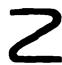
\includegraphics[keepaspectratio]{images/part003_91527dd3.jpg}}

COROLLARY 1. --- Every finitely generated module E over a principal ideal domain is the direct sum of the torsion submodule of E and a free module.

The torsion submodule of E has in general several distinct complements. For example, if \(E = \mathbf{Z} \times (\mathbf{Z}/(2))\) then the torsion submodule of E is \(\{0\} \times (\mathbf{Z}/(2))\) ; it has as a complement the submodule \(Z \times \{0\}\) , and also the submodule consisting of all elements \((n, \bar{n})\) , where n runs through Z and \(\bar{n}\) is the residue class of n mod 2.

COROLLARY 2. --- Every torsion free finitely generated module over a principal ideal domain is free of finite rank.

This follows immediately from Cor. 1.

\pandocbounded{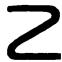
\includegraphics[keepaspectratio]{images/part003_b18cf4bc.jpg}}

The condition that the module be finitely generated is essential. For example the additive group of the field of fractions K of A is torsion free as an A-module; however it is not a free module if \(A \neq K\) , for on the one hand any two elements of K have a common divisor, and on the other hand K is not a cyclic A-module, for otherwise \(K = ab^{-1}A\) ( \(a, b \in A\) ), whence \(b^{-2} = acb^{-1}\) ( \(c \in A\) ), so \(b^{-1} = ac \in A\) , and K = A.

DEFINITION 2. --- In the notation and hypotheses of Th. 2, the ideals \(\mathfrak{a}_k\) are called the invariant factors of the module E.

As in Def. 1 (VII, p.~19), when A = Z or A = K{[}X{]}, the canonical generator of the ideal \(a_{k}\) (a positive integer or a monic polynomial) is also called, by abuse of language, an invariant factor of the finitely generated module E.

\pandocbounded{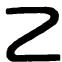
\includegraphics[keepaspectratio]{images/part003_8ba9a087.jpg}}

We must be careful not to confuse the invariant factors of a module E with those of a submodule M of a free module L with respect to the module L (Def. 1).

